\documentclass[acmsmall,screen,nonacm]{acmart}
\setcopyright{none}
\settopmatter{printfolios=true,printccs=false,printacmref=false}
\renewcommand\footnotetextcopyrightpermission[1]{}
\raggedbottom
\usepackage{microtype}
\usepackage{amsthm,mathtools}
\usepackage{enumitem}
\usepackage{xcolor}
\usepackage{listings}
\usepackage{tikz}
\usetikzlibrary{arrows.meta,positioning,calc}

\title{A Semantic Reduction from Conditional Safety to Local Proofs}
\author{Fr\'ed\'eric Dabrowski}
\affiliation{%
  \institution{Univ.Orl\'eans, INSA Centre Val de Loire, LIFO EA 4022}
  \city{Orl\'eans}
  \country{France}
}
\email{frederic.dabrowski@univ-orleans.fr}

\newtheorem{theorem}{Theorem}
\newtheorem{proposition}[theorem]{Proposition}
\newtheorem{lemma}[theorem]{Lemma}
\newtheorem{definition}[theorem]{Definition}
\newtheorem{remark}[theorem]{Remark}

\newcommand{\AvoidA}{\mathsf{Avoid}_A}
\newcommand{\AvoidG}{\mathsf{Avoid}_G}
\newcommand{\Match}{\mathsf{Match}}
\newcommand{\TransRel}{\mathsf{TransRel}}
\newcommand{\Target}{\mathsf{Target}}
\newcommand{\Valid}{\mathsf{Valid}}
\newcommand{\Generated}{\mathsf{Generated}}
\newcommand{\Ctx}{\mathsf{Ctx}}
\newcommand{\Bad}{\mathsf{Bad}}
\newcommand{\NoBad}{\mathsf{NoBad}}
\newcommand{\Coherence}{\mathsf{Coh}}
\newcommand{\NodeInv}{\mathsf{Inv}}
\newcommand{\GlobCorr}{\mathsf{GlobCorr}}
\newcommand{\InvTrue}{\mathsf{InvTrue}}
\newcommand{\CohCur}{\mathsf{Coh}^{\mathsf{cur}}}
\newcommand{\CohNext}{\mathsf{Coh}^{\mathsf{next}}}
\newcommand{\pre}{\mathsf{pre}}
\newcommand{\post}{\mathsf{post}}
\newcommand{\curS}{\mathsf{curS}}
\newcommand{\curA}{\mathsf{curA}}
\newcommand{\curG}{\mathsf{curG}}
\newcommand{\nextS}{\mathsf{nextS}}
\newcommand{\nextA}{\mathsf{nextA}}
\newcommand{\nextG}{\mathsf{nextG}}

\definecolor{kairoskw}{RGB}{11,72,107}
\definecolor{kairoscomment}{RGB}{90,90,90}
\definecolor{kairosstring}{RGB}{146,49,49}
\definecolor{kairosbg}{RGB}{248,248,248}

\lstdefinelanguage{Kairos}{
  keywords={node,returns,contracts,requires,ensures,locals,states,invariants,transitions,to,when,in,end,init},
  sensitive=true,
  morecomment=[l]{//},
  morestring=[b]"
}

\lstdefinestyle{kairosstyle}{
  language=Kairos,
  basicstyle=\ttfamily\small,
  keywordstyle=\color{kairoskw}\bfseries,
  commentstyle=\color{kairoscomment}\itshape,
  stringstyle=\color{kairosstring},
  columns=fullflexible,
  keepspaces=true,
  showstringspaces=false,
  frame=single,
  framerule=0.2pt,
  rulecolor=\color{black!20},
  backgroundcolor=\color{kairosbg},
  xleftmargin=0.4em,
  xrightmargin=0.4em,
  aboveskip=0.6em,
  belowskip=0.4em
}

\begin{document}
\begin{abstract}
\noindent\textbf{Abstract. }
We study conditional safety of reactive programs over infinite input streams and
unbounded semantic domains. The target property says that every input stream
satisfying an assumption must produce only executions satisfying a safety
guarantee. Such properties are global by nature, whereas deductive
verification is local and transition-based. We identify a canonical local proof
interface for this mismatch. Starting from the explicit product of the program
with assumption and guarantee safety automata, we localize global violations to
dangerous product steps, extract semantic clauses from these steps, and package
these clauses into relational Hoare triples over ticks. We prove that this
reduction is sound: validity of all generated triples implies conditional
safety. We also prove two relative-completeness results for the reduction
itself: global correctness implies validity of all generated safety triples,
and, under true user invariants, validity of all generated triples. The
development is formalized in Rocq. Concrete validation mechanisms are treated
only as later instantiations of this abstract proof interface.
\end{abstract}

\keywords{reactive programs, conditional safety, local proofs, relational Hoare logic, safety automata}

\maketitle

\section{Introduction}
Safety requirements for reactive programs are naturally stated over infinite
traces. In the conditional setting considered here, one does not ask that every
environment behavior be safe, but rather that every \emph{admissible} input
stream lead to a safe execution. This yields properties of the form
\[
  \text{if the input satisfies } A,\ \text{then the execution satisfies } G,
\]
where $A$ and $G$ denote safety properties. Such formulations are standard in
assume/guarantee reasoning and in synchronous verification
\cite{pnueli-1977,halbwachs-1991,berry-benveniste-sync}.

The technical difficulty is that the property is global, whereas deductive
verification proceeds locally. The state spaces of the programs of interest are
not necessarily finite, since they manipulate semantic domains such as
integers, records, or memories with user-defined structure. Direct finite-state
reasoning is therefore unavailable at the program level. At the same time,
safety properties themselves admit canonical finite representations through
safety automata and their standard constructions
\cite{alpern-schneider,kupferman-vardi-safety,gastin-oddoux}. The problem is
to connect these two levels without collapsing the semantics of the program
into a backend-specific verification-condition encoding.

This question is not merely an engineering concern. If the mathematical model
is phrased too directly in terms of a concrete verification backend, then the
semantic content of the reduction becomes hard to isolate: soundness depends on
tool-specific encodings, and completeness statements become difficult to
interpret. Conversely, if the model stays entirely at the level of global trace
properties, then it fails to explain why local proof obligations should suffice
at all. A satisfactory account should therefore expose an intermediate layer
that is simultaneously semantic, local, and backend-independent.

The non-trivial point is therefore not the mere existence of safety automata, nor the
observation that local verification conditions are useful in practice. The
non-trivial point is to identify the semantic object that makes the local proof
objects both inevitable and backend-independent. The thesis of this paper is
that the explicit product between the program and the two safety automata is
exactly this object. Once the product has been fixed, dangerous steps,
semantic clauses, and relational triples are no longer ad hoc proof artifacts:
they become the canonical local interface of the global conditional-safety
semantics.

This paper isolates a semantic answer. We define a canonical explicit product
between a reactive program and two safety automata, one for the assumption and
one for the guarantee. This product is not introduced as an implementation
artifact, but as the semantic device that localizes global violations. Once the
product is available, a global violation of the guarantee can be reduced to the
existence of a concrete tick that realizes a dangerous local product step. From
such steps we extract local semantic clauses, and from these clauses we build
relational Hoare triples over ticks. The resulting proof objects are local, but
they still retain an explicit connection to the global safety semantics.

The contribution is a small semantic theory organized around three central
results. First, validity of all generated relational triples implies
conditional safety. Second, global correctness implies validity of the
generated $\NoBad$ triples. Third, under the additional assumption that user
invariants are semantically true on executions, all generated triples are
valid. The first theorem justifies the reduction as a sound proof method; the
second and third explain why the reduction generates semantically legitimate
local proof objects rather than arbitrary artifacts.

The core theory is independent of any particular tool. In practice, one may
start from a specification language such as a safety fragment of LTL, compile
it to safety automata, and discharge the generated triples with an external
backend such as Why3 \cite{why3}. These are instantiations of the abstract
triple layer, not part of the central mathematical result.

This perspective matters. The point is not only that a concrete verifier can be
organized around products and local triples. The point is that conditional
safety admits a semantic reduction whose local proof objects are determined by
the product semantics itself. This is the level at which the paper claims
generality.

The paper should therefore be read primarily as a theorem about a reduction,
not as a description of a verification pipeline. The pipeline perspective
reappears only once the abstract triple layer has been fixed and justified.

\paragraph{Scope of the result.}
The paper proves a reduction theorem, not a complete verification pipeline. The
core result stops at the validity of relational triples generated from the
product semantics. Concrete choices such as formula syntax, encoding into a
verification-condition language, proof search, or solver orchestration belong
to later instantiation layers. This separation is deliberate: it keeps the
semantic theorem stable while allowing multiple backends to refine it.

\paragraph{Contributions.}
The paper makes four contributions. It identifies the explicit product as the
canonical semantic object that localizes conditional-safety reasoning for
reactive programs over unbounded domains. It defines semantic clauses and
relational Hoare triples as the local proof interface induced by this product.
It proves soundness and relative-completeness theorems for the resulting
reduction. Finally, it provides a mechanized Rocq development whose public
structure mirrors the mathematical argument.

The point is not merely that a verifier can be organized around products and
triples. The point is that, once the product has been fixed, the local proof
layer is mathematically determined by the semantics rather than chosen as a
backend convenience.

\paragraph{Structure of the paper.}
Section~\ref{sec:background} recalls the standard synchronous and automata
viewpoints used by the paper. Section~\ref{sec:overview} gives a running
example. Section~\ref{sec:model} defines the reactive model, conditional
safety, and the explicit product. Section~\ref{sec:reduction} introduces
semantic clauses and relational triples. Section~\ref{sec:metatheory} states
and proves the main results. Section~\ref{sec:instantiation} explains how a
concrete tool can instantiate the abstract theory. Section~\ref{sec:related}
discusses related work and Section~\ref{sec:conclusion} concludes.

\section{Background}\label{sec:background}
The paper combines four standard viewpoints that are often studied separately.
First, we adopt the synchronous view of reactive computation
\cite{berry-benveniste-sync,halbwachs-1991}: execution proceeds in discrete
ticks, and each tick transforms a current internal configuration, a memory, and
an input into a next internal configuration, a next memory, and an output.
This one-tick organization is crucial for
the rest of the paper, because it suggests from the outset that the relevant
local proof objects should relate current and next tick contexts rather than
arbitrary long prefixes.

This synchronous reading also makes clear why a purely finite-state
model-checking account is not sufficient for the class of programs considered
here. The program state may contain integers, records, or user-defined memory
structures ranging over unbounded domains. For such systems, direct finite
exploration is unavailable in general without additional abstraction,
symbolic restrictions, or specialized infinite-state techniques
\cite{bouajjani-pushdown,clarke-cegar}. This is the setting in which the paper
places its reduction: the specification side retains a finite representation
through safety automata, while the program side remains symbolic and can range
over unbounded domains.

Second, the temporal properties of interest are safety properties over infinite
traces \cite{alpern-schneider}. Safety is exactly the fragment for which global
violation admits a finite witness: once a bad event has occurred, no extension
of the execution can repair it. This is why deterministic safety automata are
the natural finite representation of the temporal component of the
specification. They compress the relevant prefix information into a finite
state and expose failure through a distinguished bad state. In the conditional
setting studied here, one automaton reads inputs and captures admissibility,
while the other reads input/output observations and captures the guarantee. In
concrete instances, these automata can come from a safety fragment of temporal
logic through standard safety-automaton constructions
\cite{kupferman-vardi-safety,gastin-oddoux}. For safety properties, this
deterministic presentation is not an ad hoc implementation choice: it is the
representation that makes finite bad prefixes explicit, and therefore matches
the intended reduction to local proofs.

Third, the intended proof style is deductive and local. The goal is not to
reason directly on whole traces, but to extract local proof obligations whose
validity suffices for the global safety statement. For this reason, the target
proof objects are not command-level Hoare triples over an imperative syntax,
but relational triples over semantic ticks. Their role is analogous to the
role of verification conditions in ordinary Hoare logic \cite{hoare-1969,
cook-1978}: they state what must hold before and after one local step. The
difference is that the ``command'' is here the semantic relation induced by one
reactive tick.

The reduction developed in the rest of the paper should therefore be read as a
bridge between these four ingredients: synchronous ticks provide the right
granularity for local reasoning, safety automata provide a finite handle on the
temporal part of the specification, conditional safety explains why two
automata are needed, and relational triples provide the deductive interface
through which the global property can be established locally.

The intended concrete instances belong to the same broad family as synchronous
intermediate languages inspired by Lustre and observer-based compilation
\cite{halbwachs-1991,lustre-v6-manual,safecomp-observers}. In such languages, a program is
already organized around an explicit memory, an explicit control structure, and
tick-wise transitions. This explains why the abstract model of the paper gives
such a central role to internal modes and local transitions.

This ordering of ideas is also the reading strategy of the paper itself. We
first fix the synchronous and safety-theoretic setting, then introduce the
product that localizes global failures, and only afterwards turn this product
into local proof objects.

\section{Overview}\label{sec:overview}
This section gives the informal picture that the formal development will make
precise. The reader should keep four objects in mind: the program, the two
safety automata, the explicit product, and the local triple extracted from a
dangerous product step.

Consider a reactive program with an integer control state
$s \in \{\mathit{Init},\mathit{Run}\}$, an integer memory cell $m$, an integer
input $x$, an integer input $r$ used as a Boolean reset flag, and an output
$y$. The initial control state is $\mathit{Init}$, and $\mathit{Run}$ is
absorbing. The intended discipline is that $r \in \{0,1\}$ and that reset
ticks carry the distinguished reinitialization value $x = 0$. At each tick, if
$r = 1$ then the program emits $0$, stores $0$ in memory, and moves to
$\mathit{Run}$; otherwise it emits either $0$ while $s=\mathit{Init}$ or the
current memory while $s=\mathit{Run}$, stores the current input for the next
tick, and again moves to $\mathit{Run}$. In pseudo-code:
\[
\begin{array}{l}
\textbf{if } r = 1 \textbf{ then } y := 0;\ m' := 0;\ s' := \mathit{Run} \\
\textbf{else if } s = \mathit{Init} \textbf{ then } y := 0;\ m' := x;\ s' := \mathit{Run} \\
\textbf{else } y := m;\ m' := x;\ s' := \mathit{Run}
\end{array}
\]

The running specification is:
\[
\begin{array}{l}
A \equiv G((r = 0 \lor r = 1) \land (r = 1 \Rightarrow x = 0)), \\
G_1 \equiv G(r = 1 \Rightarrow y = 0), \\
G_2 \equiv X\,G((r = 0 \land \mathsf{prev}(r) = 1) \Rightarrow y = 0), \\
G_3 \equiv X\,G((r = 0 \land \mathsf{prev}(r) = 0) \Rightarrow y = \mathsf{prev}(x)).
\end{array}
\]
The aggregate guarantee is the conjunction of $G_1$, $G_2$, and $G_3$. The
user invariant attached to `Run' is likewise split into two cases:
\[
(\mathsf{prev}(r) = 1 \Rightarrow m = 0)
\land
(\mathsf{prev}(r) = 0 \Rightarrow m = \mathsf{prev}(x)).
\]
This same structure will later be instantiated in a concrete specification
language.

\begin{figure}[t]
\centering
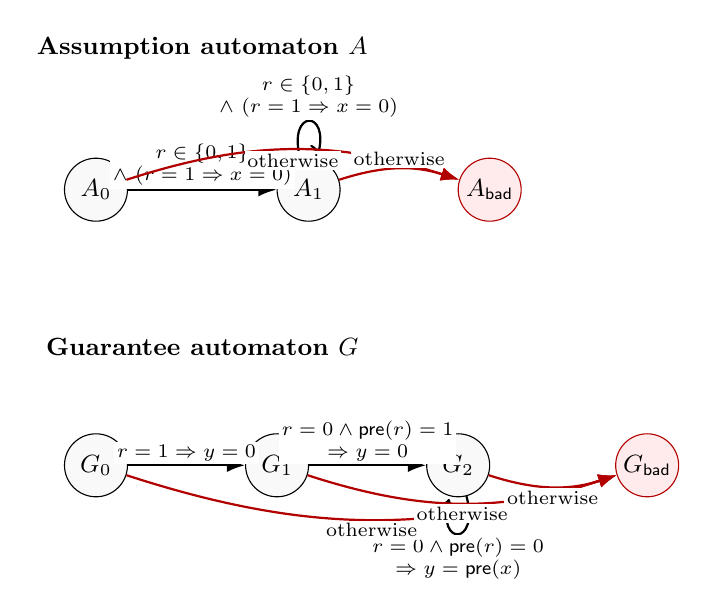
\begin{tikzpicture}[
  every node/.style={font=\small},
  aut/.style={draw,circle,minimum size=8mm,inner sep=1pt,fill=gray!5},
  bad/.style={draw,circle,minimum size=8mm,inner sep=1pt,fill=red!8,draw=red!70!black},
  arr/.style={-Latex,thick},
  lab/.style={fill=white,inner sep=1pt,font=\scriptsize,align=center}
]
  \node[align=center,font=\small\bfseries] at (1.35,1.8) {Assumption automaton $A$};
  \node[aut] (a0) at (0,0) {$A_0$};
  \node[aut] (a1) at (2.7,0) {$A_1$};
  \node[bad] (abad) at (5.0,0) {$A_{\mathsf{bad}}$};
  \draw[arr] (a0) -- node[lab,above] {$r \in \{0,1\}$\\$\land$ $(r=1 \Rightarrow x=0)$} (a1);
  \draw[arr] (a1) edge[loop above] node[lab] {$r \in \{0,1\}$\\$\land$ $(r=1 \Rightarrow x=0)$} (a1);
  \draw[arr,draw=red!70!black] (a0) to[bend left=18] node[lab,below] {otherwise} (abad);
  \draw[arr,draw=red!70!black] (a1) to[bend left=18] node[lab,above] {otherwise} (abad);

  \node[align=center,font=\small\bfseries] at (1.35,-2.0) {Guarantee automaton $G$};
  \node[aut] (g0) at (0,-3.5) {$G_0$};
  \node[aut] (g1) at (2.3,-3.5) {$G_1$};
  \node[aut] (g2) at (4.6,-3.5) {$G_2$};
  \node[bad] (gbad) at (7.0,-3.5) {$G_{\mathsf{bad}}$};
  \draw[arr] (g0) -- node[lab,above] {$r=1 \Rightarrow y=0$} (g1);
  \draw[arr] (g1) -- node[lab,above] {$r=0 \land \pre(r)=1$\\$\Rightarrow y=0$} (g2);
  \draw[arr] (g2) edge[loop below] node[lab] {$r=0 \land \pre(r)=0$\\$\Rightarrow y=\pre(x)$} (g2);
  \draw[arr,draw=red!70!black] (g0) to[bend right=18] node[lab,below] {otherwise} (gbad);
  \draw[arr,draw=red!70!black] (g1) to[bend right=18] node[lab,below] {otherwise} (gbad);
  \draw[arr,draw=red!70!black] (g2) to[bend right=18] node[lab,below] {otherwise} (gbad);
\end{tikzpicture}
\caption{Safety automata for the running example. The assumption automaton
tracks the reset discipline, while the guarantee automaton distinguishes reset
ticks, the first non-reset tick after reset, and the ordinary one-step delay
case.}
\Description{Two small safety automata for the running example. The first one
checks the reset discipline on inputs, and the second one checks the three
guarantee cases on input-output observations.}
\label{fig:running-automata}
\end{figure}

The proof method does not start by generating verification conditions directly
from the source program. Instead, it forms the product of the program with a
safety automaton for the assumption and a safety automaton for the guarantee. A
concrete tick then determines a concrete program transition and advances both
automata. The key local notion is that of a \emph{dangerous step}: a product
step that remains admissible for the assumption automaton but moves the
guarantee automaton into its bad state.

This dangerous step is the pivot of the reduction. It is the local event that
witnesses a global guarantee violation. Once such a step has been identified,
the reduction does two things. First, it extracts a semantic safety clause
$\NoBad$ stating that the current tick does not realize that step. Second, it
packages this clause into a local relational triple whose precondition
contains exactly the coherence information needed to make the safety clause
meaningful.

The coherence layer is part of the reduction, not an external proof heuristic.
Some coherence triples transport user invariants. Others transport the fact
that the current concrete tick is coherent with the current abstract product
state. Safety triples and coherence triples therefore live in the same local
proof world: the latter provide the local context in which the former can
exclude dangerous concrete steps.

The point of the example is not that its local proof obligations are difficult,
but that the reduction separates three levels cleanly. At the trace level, the
property is conditional safety. At the product level, violations become
dangerous local steps. At the triple level, dangerous steps become local proof
objects whose preconditions contain exactly the coherence information needed
for local reasoning. The same pattern will be used in the general theory, and
Section~\ref{sec:instantiation} will return to this example in a concrete
specification language.

\paragraph{A concrete dangerous case.}
Suppose the current tick is a non-reset tick with $\mathsf{prev}(r) = 0$, so
the active guarantee branch is $G_3$ and the expected output is
$\mathsf{prev}(x)$. If the local context records a transition whose concrete
output disagrees with that value, then the guarantee automaton moves to its bad
state while the assumption automaton may still remain admissible, since the
Boolean/reset discipline can still hold. This yields a dangerous product step.
The associated safety clause simply says that the current context must not
realize this step. The corresponding safety triple is local, but its
justification still depends on two kinds of coherence facts: the user
invariant that explains the meaning of $m$ in the current reset mode, and the
automaton coherence fact that identifies the current abstract product state.

\begin{figure}[t]
\centering
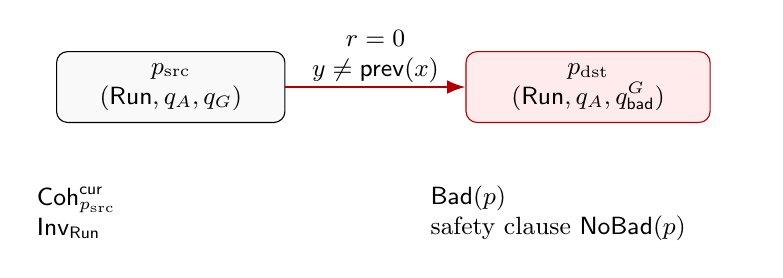
\begin{tikzpicture}[
  every node/.style={font=\small},
  pstate/.style={draw,rounded corners,minimum width=2.9cm,minimum height=0.9cm,align=center,fill=gray!5},
  badstate/.style={draw,rounded corners,minimum width=3.1cm,minimum height=0.9cm,align=center,fill=red!8,draw=red!70!black},
  arr/.style={-Latex,thick},
  darr/.style={-Latex,thick,draw=red!70!black}
]
\node[pstate] (src) at (0,0) {$p_{\mathrm{src}}$\\$(\mathsf{Run},q_A,q_G)$};
\node[badstate] (dst) at (5.3,0) {$p_{\mathrm{dst}}$\\$(\mathsf{Run},q_A,q^G_{\mathsf{bad}})$};
\draw[darr] (src) -- node[above,align=center,fill=white,inner sep=1pt]
  {$r=0$\\$y \neq \mathsf{prev}(x)$} (dst);
\node[align=left,text width=3.4cm] at (0,-1.6)
  {$\CohCur_{p_{\mathrm{src}}}$\\$\NodeInv_{\mathsf{Run}}$};
\node[align=left,text width=4.0cm] at (5.3,-1.6)
  {$\Bad(p)$\\safety clause $\NoBad(p)$};
\end{tikzpicture}
\caption{Relevant fragment of the explicit product for the running example.
The red edge is a dangerous step: if a concrete tick matches it, the generated
triple $h^{\NoBad}(p)$ is activated.}
\Description{A fragment of the running explicit product with a source product
state, a dangerous edge labelled by a non-reset mismatch, and a target product
state whose guarantee component is bad. The figure also recalls the source
coherence and invariant facts and the associated safety clause.}
\label{fig:dangerous-fragment}
\end{figure}

\paragraph{What the overview already shows.}
Even before the formal definitions, the example exhibits the full proof
architecture. A global violation of the guarantee is localized to one concrete
tick. The local context of that tick identifies a dangerous product step. This
step generates a semantic safety clause. The clause is embedded into a local
triple whose precondition is built from coherence information. The rest of the
paper turns this informal picture into a general semantic reduction theorem:
\[
  \text{valid generated local triples}
  \Longrightarrow
  \text{conditional safety.}
\]

\begin{center}
\begin{tabular}{@{}l@{}}
\textbf{Reduction at a glance} \\
1. A global guarantee violation yields a dangerous product step. \\
2. That step yields one local safety clause $\NoBad(p)$. \\
3. The clause is packaged into one local safety triple $h^{\NoBad}(p)$. \\
4. Coherence triples justify the local preconditions of $h^{\NoBad}(p)$. \\
5. Valid generated triples therefore imply conditional safety. \\
\end{tabular}
\end{center}

The formal development below simply turns each line of this summary into a
definition or theorem. The running example keeps reappearing so that the reader
never has to reconstruct the intended local picture from the abstract
definitions alone.

\section{Semantic Model}\label{sec:model}

The purpose of this section is not to introduce yet another operational model,
but to isolate the smallest semantic structure needed by the reduction. We
need a notion of reactive tick, a notion of safety automaton over infinite
streams, and a product that makes one local step carry exactly the information
needed by the local proof interface. Each definition below should therefore be
read as introducing one piece of this interface.

\subsection{Reactive programs}
\paragraph{Intuition.}
The reduction does not depend on a concrete source syntax. What matters is only
that one reactive tick can be observed semantically: from a current internal
state, a current memory, and a current input, the program chooses a transition
and produces a successor state, a successor memory, and an output. The formal
notion of control state is introduced just below; before that point, it can be
read simply as the abstract mode in which the program currently operates. We
package this directly as semantic data.

\begin{definition}[Reactive program]
A reactive program is a tuple
\[
  P = (S,M,I,O,T,s_0,\mathsf{select},\mathsf{enabled},\mathsf{dst},\mathsf{upd},\mathsf{out})
\]
where $S$, $M$, $I$, $O$, and $T$ are respectively the control-state,
memory, input, output, and transition spaces; $s_0 \in S$ is the initial
control state; and
\begin{align*}
  \mathsf{select} &: S \times M \times I \to T,\\
  \mathsf{enabled} &: T \times S \times M \times I \to \mathsf{Prop},\\
  \mathsf{dst} &: T \times S \to S,\\
  \mathsf{upd} &: T \times M \times I \to M,\\
  \mathsf{out} &: T \times M \times I \to O.
\end{align*}
The selected transition is always enabled:
\[
  \forall s \in S,\forall m \in M,\forall i \in I,\quad
  \mathsf{enabled}(\mathsf{select}(s,m,i),s,m,i).
\]
\end{definition}

The theory is intentionally extensional: it does not assume a command syntax,
a control-flow graph, or a verification-condition generator, but only the
semantic data needed to describe one reactive tick. By construction, programs
in this model are total at the level of one tick: for every current control
state, current memory, and current input, the model provides a selected
transition, a successor control state, a successor memory, and an output.

\begin{definition}[Execution from an initial memory]
Fix a program $P$, an input stream $u : \mathbb{N} \to I$, and an initial
memory $m_0 \in M$. The execution of $P$ from $m_0$ on $u$ is the tuple of
streams $(s_u,m_u,t_u,o_u)$ defined by:
\[
  s_u(0) = s_0,\qquad m_u(0)=m_0,
\]
and, for every $k \in \mathbb{N}$,
\begin{align*}
  t_u(k) &= \mathsf{select}(s_u(k), m_u(k), u(k)),\\
  o_u(k) &= \mathsf{out}(t_u(k), m_u(k), u(k)),\\
  s_u(k+1) &= \mathsf{dst}(t_u(k), s_u(k)),\\
  m_u(k+1) &= \mathsf{upd}(t_u(k), m_u(k), u(k)).
\end{align*}
\end{definition}

\paragraph{Running example.}
For \textsc{resettable-delay}, the control state space is
$S=\{\mathsf{Init},\mathsf{Run}\}$, the memory space is the integer domain, the
inputs are pairs $(r,x)$ made of a reset flag and an integer, and the output is
an integer $y$. On reset ticks ($r=1$), the program emits $0$ and stores $0$.
On non-reset ticks, it emits the current memory and stores the current input
$x$, except for the first non-reset tick in state $\mathsf{Init}$, where it
emits $0$ and moves to $\mathsf{Run}$.

\subsection{Conditional safety}
\paragraph{Intuition.}
The program alone is not enough: the property is conditional. One automaton
filters admissible inputs; the other checks whether the observable
input/output behavior remains safe. Since we focus on safety, both automata are
deterministic safety automata with a distinguished bad state.

\begin{definition}[Deterministic safety automaton]
For an alphabet $X$, a deterministic safety automaton is a tuple
\[
  \mathcal{A} = (Q,q_0,q_{\mathsf{bad}},\delta)
\]
where $Q$ is a state space, $q_0 \in Q$ is the initial state,
$q_{\mathsf{bad}} \in Q$ is the bad state, and
$\delta : Q \times X \to Q$ is a deterministic step function.
\end{definition}

Thus safety automata are total at the level of one letter: for every current
state and every current observation, the next automaton state is defined by
the function $\delta$.

\begin{definition}[Run and safety acceptance]
Let $\mathcal{A}=(Q,q_0,q_{\mathsf{bad}},\delta)$ be a deterministic safety
automaton over $X$, and let $w : \mathbb{N} \to X$ be an infinite word. The
run of $\mathcal{A}$ on $w$ is the stream $q_w : \mathbb{N} \to Q$ defined by
\[
  q_w(0)=q_0,\qquad q_w(k+1)=\delta(q_w(k),w(k)).
\]
We say that $\mathcal{A}$ accepts $w$ when
\[
  \forall k.\ q_w(k) \neq q_{\mathsf{bad}}.
\]
\end{definition}

The assumption automaton is written
\[
  A=(Q_A,q^A_0,q^A_{\mathsf{bad}},\delta_A)
\]
and reads inputs in $I$. The guarantee automaton is written
\[
  G=(Q_G,q^G_0,q^G_{\mathsf{bad}},\delta_G)
\]
and reads observable input-output pairs in $I \times O$. For an internal run
from $m_0$ on input stream $u$, the observable trace is
\[
  \tau_{m_0,u}(k) = (u(k), o_u(k)).
\]
The conditional specification additionally assumes that the initial states of
both automata are not already bad:
\[
  q^A_0 \neq q^A_{\mathsf{bad}}
  \qquad\text{and}\qquad
  q^G_0 \neq q^G_{\mathsf{bad}}.
\]

\begin{definition}[Conditional safety predicates]
\begin{align*}
  \AvoidA(u) &\triangleq
    \forall k \in \mathbb{N}.\ q^A_u(k) \neq q^A_{\mathsf{bad}},\\
  \AvoidG(u) &\triangleq
    \forall m_0 \in M,\forall k \in \mathbb{N}.\ q^G_{m_0,u}(k) \neq q^G_{\mathsf{bad}}.
\end{align*}
\end{definition}

\paragraph{Running example.}
In \textsc{resettable-delay}, the assumption automaton checks the input-side
discipline $r \in \{0,1\}$ and $r=1 \Rightarrow x=0$. The guarantee automaton
checks three safety branches: reset ticks emit $0$, the first non-reset tick
after a reset emits $0$, and ordinary non-reset ticks emit the previous
non-reset input. Thus $\AvoidA(u)$ means that the input stream respects the
reset discipline, whereas $\AvoidG(u)$ means that every execution on $u$
respects all three branches of the intended delay behavior.

The distinction between assumption and guarantee is crucial. The assumption
automaton constrains which inputs are semantically relevant, whereas the
guarantee automaton constrains which observable input/output traces are
acceptable for the program. The core theorem is therefore a theorem of
conditional safety, not of unconditional trace acceptance.

\subsection{Explicit product}
\paragraph{Intuition.}
At this point one could try to reason directly on executions and automaton runs,
but that would keep the safety argument global. The product is introduced
precisely to make one local tick carry the program state and the two automaton
states at once. It is the object on which ``dangerous local step'' becomes a
 meaningful notion.

\begin{definition}[Product state]
A product state is a triple
\[
  p=(s,q_A,q_G)\in S \times Q_A \times Q_G.
\]
We write $\pi_S(p)=s$, $\pi_A(p)=q_A$, and $\pi_G(p)=q_G$ for its three
projections.
\end{definition}

\begin{definition}[Product state along an execution]
Fix $m_0$ and $u$. Let $q^A_u$ be the run of $A$ on $u$, and let $q^G_{m_0,u}$
be the run of $G$ on $\tau_{m_0,u}$. The product state at tick $k$ is
\[
  \mathsf{pst}_{m_0,u}(k) \triangleq
  (s_u(k), q^A_u(k), q^G_{m_0,u}(k)).
\]
\end{definition}

\begin{definition}[Product step]
A product step is a tuple
\[
  p = (p_{\mathrm{src}}, t, m, i, o, p_{\mathrm{dst}})
\]
where $p_{\mathrm{src}}$ and $p_{\mathrm{dst}}$ are product states,
$t \in T$, $m \in M$, $i \in I$, and $o \in O$.
\end{definition}

Thus a product step records one program tick together with the current memory
and observation, and with the source and target states induced in the product.

\begin{definition}[Product-step target]
For a source product state $p_{\mathrm{src}}=(s,q_A,q_G)$, a transition
$t \in T$, a memory $m \in M$, an input $i \in I$, and an output $o \in O$, we
define
\[
  \Target(p_{\mathrm{src}},t,m,i,o)
  \triangleq
  (\mathsf{dst}(t,s), \delta_A(q_A,i), \delta_G(q_G,(i,o))).
\]
\end{definition}

\begin{definition}[Selected product step]
Fix $m_0 \in M$, an input stream $u$, and a tick $k \in \mathbb{N}$. The
selected product step at tick $k$ is
\[
  \mathsf{step}_{m_0,u}(k) \triangleq
  (\mathsf{pst}_{m_0,u}(k), t_u(k), m_u(k), u(k), o_u(k), \mathsf{pst}_{m_0,u}(k+1)).
\]
\end{definition}

\paragraph{Running example.}
In the running example, a product state records one control state
($\mathsf{Init}$ or $\mathsf{Run}$), one assumption-automaton state, and one
guarantee-automaton state. A product step for a non-reset tick in
$\mathsf{Run}$ records not only the source and target automaton states, but also
the current memory $m$, the current input $(r,x)$ with $r=0$, and the emitted
output $y=m$. This is precisely the information needed to decide whether the
guarantee branch ``ordinary delay'' is respected locally.

The explicit product is finite as soon as $S$, $Q_A$, and $Q_G$ are finite.
Memory and observations are not folded into the product state; they are carried
only by local product steps and local tick contexts.

\subsection{Local tick contexts and matching}
\paragraph{Intuition.}
The product step is still an abstract object. To connect it to actual
executions, we need a local semantic snapshot of one concrete tick. This is the
role of the tick context: it records the current configuration, the current
observation, the selected transition, and the immediate successor
configuration. Matching is then the bridge between a concrete tick and an
abstract product step.

\begin{definition}[Tick context]
Fix $m_0$, $u$, and $k$. The tick context at tick $k$ is
\[
  \Ctx_{m_0,u}(k) \triangleq
  (\curS, m_u(k), u(k), o_u(k), t_u(k), \curA, \curG,
   \nextS, m_u(k+1), \nextA, \nextG)
\]
with
\begin{align*}
  \curS &= s_u(k),            & \curA &= q^A_u(k),            & \curG &= q^G_{m_0,u}(k), \\
  \nextS &= s_u(k+1),         & \nextA &= q^A_u(k+1),         & \nextG &= q^G_{m_0,u}(k+1).
\end{align*}
We reuse the symbols $\curS,\curA,\curG,\nextS,\nextA,\nextG$ for the
corresponding coordinate projections on arbitrary tick contexts.
\end{definition}

This context is the local semantic object inspected by clauses and triples: it
contains exactly the current configuration, the transition chosen at the
current tick, and the immediate successor information needed to speak about the
next product state. The context is deliberately local: the reduction never
manipulates complete execution prefixes explicitly, but packages into one
object the exact amount of concrete information that one local proof step is
allowed to inspect.

\begin{definition}[Matching]
Let
\[
  p=(p_{\mathrm{src}}, t, m, i, o, p_{\mathrm{dst}}).
\]
We say that the tick context $\Ctx_{m_0,u}(k)$ matches $p$, written
$\Match(\Ctx_{m_0,u}(k),p)$, when the following equalities hold:
\begin{align*}
  p_{\mathrm{src}} &= \mathsf{pst}_{m_0,u}(k), & t &= t_u(k), & m &= m_u(k), \\
  i &= u(k),                                   & o &= o_u(k),
\end{align*}
and
\[
  p_{\mathrm{dst}} = \mathsf{pst}_{m_0,u}(k+1).
\]
\end{definition}

The output component is essential: without it, the target guarantee state of
the product step would not be determined by the local context.

\begin{definition}[Dangerous step]
A product step
$p=(p_{\mathrm{src}}, t, m, i, o, p_{\mathrm{dst}})$ with
$p_{\mathrm{dst}}=(s',q'_A,q'_G)$ is dangerous when
\[
  q'_G = q^G_{\mathsf{bad}}
  \qquad\text{and}\qquad
  q'_A \neq q^A_{\mathsf{bad}}.
\]
We write $\Bad(p)$ for this predicate.
\end{definition}

\begin{definition}[Well-formed product step]
For
\[
  p=(p_{\mathrm{src}}, t, m, i, o, p_{\mathrm{dst}}),
\]
we define $\mathsf{WFStep}(p)$ by
\[
  p_{\mathrm{dst}} = \Target(p_{\mathrm{src}},t,m,i,o).
\]
\end{definition}

Thus $\mathsf{WFStep}(p)$ is a structural consistency condition on the step
itself. Realization on a concrete execution is expressed separately by the
matching predicate $\Match$.

\paragraph{Running example.}
The canonical dangerous case is a non-reset tick in state $\mathsf{Run}$ where
the assumption still accepts the current input, but the guarantee moves to its
bad state because the emitted value does not agree with the previous
non-reset input. In that case the product step is dangerous exactly because the
assumption remains admissible while the guarantee fails.

\begin{proposition}[Global violation yields a dangerous step]
\label{prop:global-to-dangerous}
Let $m_0 \in M$, and let $u$ be an input stream. If
\[
  \AvoidA(u)
  \qquad\text{and}\qquad
  \exists j \in \mathbb{N}.\ q^G_{m_0,u}(j) = q^G_{\mathsf{bad}},
\]
then there exists a tick $k \in \mathbb{N}$ such that
\[
  \Bad(\mathsf{step}_{m_0,u}(k)).
\]
\end{proposition}

\noindent
This proposition is the semantic localization principle: it reduces a global
violation of the guarantee to a concrete local event.

\begin{proof}[Proof idea]
If the guarantee automaton reaches its bad state on an execution,
then there is a first tick at which the bad state is entered. The current
program state, the current automaton states, the selected program transition,
and the current observation determine a concrete product step. By construction,
its target guarantee state is bad. Since the assumption still holds on the run,
the target assumption state is not bad. Therefore the realized product step is
dangerous.
\end{proof}

\section{Reduction to Local Proofs}\label{sec:reduction}

The reduction has two layers. First, dangerous product steps induce semantic
clauses that describe what must be ruled out or propagated locally. Second,
these clauses are assembled into relational triples, which are the actual local
proof objects. The distinction matters: clauses carry the semantic content of
the reduction, while triples provide the local proof interface.

\subsection{Semantic clauses}
\paragraph{Intuition.}
Clauses are the smallest semantic facts extracted from the product. Safety
clauses prohibit dangerous concrete realizations. Invariant clauses record
semantic information supplied by the specification. Coherence clauses say which
abstract product state the current or next concrete tick corresponds to.

\begin{definition}[Semantic clause]
A semantic clause is a predicate
\[
  C : \Ctx \to \mathsf{Prop}.
\]
\end{definition}

We use three canonical families of clauses.

\begin{definition}[Safety clause]
For a dangerous product step $p$, the safety clause generated by $p$ is
\[
  \NoBad(p)(\Ctx) \triangleq \neg \Match(\Ctx,p).
\]
\end{definition}

\begin{definition}[User-invariant clause]
For a control state $s \in S$, the user-invariant clause attached to $s$ is a
semantic predicate
\[
  \NodeInv_s : \Ctx \to \mathsf{Prop}.
\]
In the abstract theory, these predicates are part of the specification rather
than part of the program semantics.
\end{definition}

\begin{definition}[Automaton-coherence clauses]
Let $p=(s,q_A,q_G)$ be a product state. The current coherence clause and next
coherence clause attached to $p$ are the predicates
\[
  \CohCur_p(\Ctx) \triangleq
  (\curS(\Ctx)=s \wedge \curA(\Ctx)=q_A \wedge \curG(\Ctx)=q_G),
\]
\[
  \CohNext_p(\Ctx) \triangleq
  (\nextS(\Ctx)=s \wedge \nextA(\Ctx)=q_A \wedge \nextG(\Ctx)=q_G).
\]
\end{definition}

These clauses are semantic, not syntactic: they state directly that the current
or next part of the tick context corresponds to a given abstract product state.
This is why the automaton-coherence part of the theory does not require an
extra correctness hypothesis about generated support formulas.

\subsection{Relational Hoare triples}
\paragraph{Intuition.}
The local proof interface is not a syntax-directed Hoare logic for commands.
Instead, each generated proof obligation talks about one semantic tick. The
precondition constrains the current context, the postcondition constrains the
next one, and the target tells us which initial or one-step semantic situation
the triple talks about.

The actual local proof objects are relational Hoare triples. A triple is
attached either to the initial tick or to a concrete program transition.

\begin{definition}[Relational Hoare triple]
A relational Hoare triple is a tuple
\[
  h = (\mathit{target}, \mathit{pre}, \mathit{post})
\]
where $\mathit{target}$ is either the distinguished initial tick or a program
transition $t \in T$, and where $\mathit{pre}$ and $\mathit{post}$ are
semantic clauses.
\end{definition}

We use $\top$ and $\bot$ for the always-true and always-false semantic
clauses.

\begin{definition}[Transition relation of a program transition]
For a transition $t \in T$, we define
\[
  \TransRel_t(\Ctx,\Ctx') \triangleq
  \exists m_0 \in M,\exists u : \mathbb{N} \to I,\exists k \in \mathbb{N},
\]
\[
  \Ctx = \Ctx_{m_0,u}(k)
  \wedge
  \Ctx' = \Ctx_{m_0,u}(k+1)
  \wedge
  t_u(k) = t.
\]
\end{definition}

\begin{definition}[Triple validity]
\[
  \Valid((\mathit{init},\pre,\post))
  \triangleq
  \forall m_0 \in M,\forall u : \mathbb{N} \to I,\
  \pre(\Ctx_{m_0,u}(0)) \rightarrow \post(\Ctx_{m_0,u}(0)).
\]
For a step triple with target transition $t \in T$, we define
\[
  \Valid((t,\pre,\post))
  \triangleq
  \forall \Ctx,\Ctx'.\
  \TransRel_t(\Ctx,\Ctx') \wedge \pre(\Ctx)
  \Longrightarrow \post(\Ctx').
\]
\end{definition}

This is a relational form of Hoare reasoning rather than an imperative one. The
triple does not interpret a command syntax. Instead, it constrains the semantic
transition relation induced by one program tick. In set-theoretic terms, if
$R_t$ is the relation associated with transition $t$, then validity expresses
that $R_t$ maps the set denoted by the precondition into the set denoted by the
postcondition. This distinction matters for readability as well as for theory:
the paper is not proposing a new command language or a new
verification-condition calculus, but identifying the semantic shape of the
local proof obligations that any concrete backend will later refine.

\paragraph{Running example.}
For the dangerous non-reset \texttt{Run}-step of \textsc{resettable-delay}, the
corresponding safety triple has a precondition saying: the current context
matches this step, the current product state is indeed the expected one, and
the user invariant attached to \texttt{Run} holds. Its postcondition is
$\bot$. This is the local proof object that excludes the concrete mismatch
$y \neq \mathsf{prev}(x)$.

\subsection{Generated triples}
\paragraph{Intuition.}
The generated triples are not an arbitrary menu of local proof obligations. The
initial triples establish the facts that must already hold at the first tick.
The propagation triples say how these facts move from one tick to the next. The
safety triples then use exactly these facts to rule out dangerous concrete
realizations. The five families below should therefore be read as the minimal
closure of the reduction under initialization, propagation, and local safety.

\begin{definition}[Canonical generated triples]
Let
\[
  p_0 \triangleq (s_0,q^A_0,q^G_0)
\]
be the initial product state. The reduction uses the following canonical
triples:
\begin{align*}
  h^{\mathsf{init}}_{\NodeInv} &\triangleq
    (\mathit{init},\top,\NodeInv_{\pi_S(p_0)}),\\
  h^{\mathsf{init}}_{\Coherence} &\triangleq
    (\mathit{init},\top,\CohCur_{p_0}).
\end{align*}
For every well-formed product step
\[
  p=(p_{\mathrm{src}},t,m,i,o,p_{\mathrm{dst}}),
\]
we define
\begin{align*}
  h^{\mathsf{prop}}_{\NodeInv}(p) &\triangleq
    \bigl(
      t,\
      \lambda \Ctx.\ \Match(\Ctx,p)
        \wedge \NodeInv_{\pi_S(p_{\mathrm{src}})}(\Ctx)
        \wedge \CohCur_{p_{\mathrm{src}}}(\Ctx),\
      \NodeInv_{\pi_S(p_{\mathrm{dst}})}
    \bigr),\\
  h^{\mathsf{prop}}_{\Coherence}(p) &\triangleq
    \bigl(
      t,\
      \lambda \Ctx.\ \Match(\Ctx,p)\wedge \CohCur_{p_{\mathrm{src}}}(\Ctx),\
      \CohCur_{p_{\mathrm{dst}}}
    \bigr).
\end{align*}
For every dangerous well-formed product step $p$, we define
\[
  h^{\NoBad}(p) \triangleq
  \bigl(
    t,\
    \lambda \Ctx.\ \Match(\Ctx,p)
      \wedge \NodeInv_{\pi_S(p_{\mathrm{src}})}(\Ctx)
      \wedge \CohCur_{p_{\mathrm{src}}}(\Ctx),\
    \bot
  \bigr).
\]
\end{definition}

The safety clause $\NoBad(p)$ is therefore not itself the postcondition of the
safety triple. Rather, it is the semantic content enforced by the triple: if
the precondition of $h^{\NoBad}(p)$ holds at a tick, then no successor context
can exist, so the current context cannot realize the dangerous step $p$. The
two propagation families are coherence triples. They establish the local facts
needed by the safety triples, so user invariants and automaton coherence are
transported in the same local proof contexts rather than in two independent
proof phases.

\begin{definition}[Generated triples]
\begin{align*}
  \Generated(h) \triangleq{}&
    h = h^{\mathsf{init}}_{\NodeInv}
    \ \vee\
    h = h^{\mathsf{init}}_{\Coherence}\\
  &\vee\ \exists p.\ \mathsf{WFStep}(p) \wedge h = h^{\mathsf{prop}}_{\NodeInv}(p)\\
  &\vee\ \exists p.\ \mathsf{WFStep}(p) \wedge h = h^{\mathsf{prop}}_{\Coherence}(p)\\
  &\vee\ \exists p.\ \mathsf{WFStep}(p) \wedge \Bad(p) \wedge h = h^{\NoBad}(p),
\end{align*}
and
\[
  \Generated_{\NoBad}(h) \triangleq
  \exists p.\ \mathsf{WFStep}(p) \wedge \Bad(p) \wedge h = h^{\NoBad}(p).
\]
\end{definition}

\paragraph{Running example.}
For \textsc{resettable-delay}, the generated initialization triples establish
the invariant and automaton coherence facts at the first tick. The propagation
triples transport these facts across reset and non-reset transitions. Finally,
the safety triples forbid exactly the dangerous local situations identified in
the product, such as a non-reset $\mathsf{Run}$ step whose output disagrees
with the delayed input expected by the guarantee automaton.

It is useful to make the partition explicit. The reduction generates exactly
five families:
\[
\begin{array}{rcl}
h^{\mathsf{init}}_{\NodeInv}
  &:& \text{initial user-invariant triple},\\
h^{\mathsf{init}}_{\Coherence}
  &:& \text{initial automaton-coherence triple},\\
h^{\mathsf{prop}}_{\NodeInv}(p)
  &:& \text{propagation of the user invariant along } p,\\
h^{\mathsf{prop}}_{\Coherence}(p)
  &:& \text{propagation of product-state coherence along } p,\\
h^{\NoBad}(p)
  &:& \text{local safety triple for a dangerous step } p.
\end{array}
\]
For the running example, the first four families establish and propagate the
local facts needed to interpret the delayed-output requirement, while the last
family excludes precisely the dangerous case highlighted in
Figure~\ref{fig:dangerous-fragment}.

This is the point at which the reduction becomes easy to read operationally.
The two initialization triples explain how the local proof context starts; the
two propagation families explain how that context survives from one tick to the
next; and the safety family then uses exactly this accumulated local context to
exclude the dangerous product steps singled out by the explicit product. So the
reduction is not merely “generate some local proof obligations”: it generates a
small fixed vocabulary of proof obligations, each with a specific semantic role
to initialize, propagate, or exclude one dangerous local case.

\section{Meta-Theory}\label{sec:metatheory}

The metatheory is organized around one main theorem and two adequacy
theorems. The main theorem is soundness: validity of the generated local
triples implies conditional safety. The adequacy theorems explain why the
reduction is non-degenerate: under the appropriate semantic assumptions, the
generated triples are themselves valid. The proof proceeds through a short
chain of intermediate facts that correspond to the essential conceptual steps
of the reduction.

The proof boundary is also explicit. The semantic core assumes only the truth
of the generated triples when proving soundness, and only the truth of user
invariants when proving full relative completeness. No statement in this
section depends on a concrete backend encoding, on a solver, or on a
verification-condition language.

The structure is intentionally simple. First, one shows that every concrete
tick matches the product step selected at that tick. Second, one shows that a
realized step is structurally well formed. Third, one shows that the coherence
facts carried by the local proof layer hold on executions. Fourth, one shows
that a dangerous realized step activates the precondition of the corresponding
safety triple. From there, soundness and relative completeness follow with
little additional machinery.

\paragraph{Reading guide.}
The main theorem can be read backwards. To prove conditional safety, one assumes
for contradiction that a guarantee violation occurs. Proposition
\ref{prop:global-to-dangerous} turns this global violation into one dangerous
local step. The matching and coherence lemmas then show that the local
precondition of the corresponding safety triple is indeed satisfied. Since the
triple is valid, its postcondition $\bot$ cannot hold of any concrete
successor, yielding the contradiction. The adequacy theorems later explain why
the generated triples are not arbitrary local artifacts.

It is useful to read this section with two questions in mind: why local triple
validity suffices for global conditional safety, and why the generated local
triples are semantically legitimate once the global property is already known
to hold.

\begin{lemma}[Selected steps match the current context]
\label{lem:matching}
For every $m_0 \in M$, every input stream $u$, and every tick
$k \in \mathbb{N}$,
\[
  \Match(\Ctx_{m_0,u}(k), \mathsf{step}_{m_0,u}(k)).
\]
\end{lemma}

\begin{proof}[Proof idea]
By definition, the selected product step at tick $k$ is
\[
  \mathsf{step}_{m_0,u}(k)=
  (\mathsf{pst}_{m_0,u}(k), t_u(k), m_u(k), u(k), o_u(k), \mathsf{pst}_{m_0,u}(k+1)).
\]
The tick context $\Ctx_{m_0,u}(k)$ contains exactly the same current
components: current program state, current memory, current input, current
output, current selected transition, and the current and next product-state
coordinates. Therefore every equality required by the definition of
$\Match(\Ctx_{m_0,u}(k),\mathsf{step}_{m_0,u}(k))$ holds by direct unfolding of
the definitions.
\end{proof}

\begin{lemma}[Realized steps are well formed]
\label{lem:realized-wf}
For every $m_0 \in M$, every input stream $u$, every tick $k \in \mathbb{N}$,
and every product step $p$, if
\[
  \Match(\Ctx_{m_0,u}(k),p),
\]
then
\[
  \mathsf{WFStep}(p).
\]
\end{lemma}

\begin{proof}[Proof idea]
Assume $\Match(\Ctx_{m_0,u}(k),p)$ for
\[
  p=(p_{\mathrm{src}}, t, m, i, o, p_{\mathrm{dst}}).
\]
By definition of matching, we have
\[
  p_{\mathrm{src}}=\mathsf{pst}_{m_0,u}(k),\qquad
  t=t_u(k),\qquad
  m=m_u(k),\qquad
  i=u(k),\qquad
  o=o_u(k),
\]
and
\[
  p_{\mathrm{dst}}=\mathsf{pst}_{m_0,u}(k+1).
\]
But by definition of the product-state run,
\[
  \mathsf{pst}_{m_0,u}(k+1)=
  \Target(\mathsf{pst}_{m_0,u}(k), t_u(k), m_u(k), u(k), o_u(k)).
\]
Replacing the current quantities by the corresponding components of $p$ gives
\[
  p_{\mathrm{dst}}=\Target(p_{\mathrm{src}},t,m,i,o),
\]
which is exactly $\mathsf{WFStep}(p)$.
\end{proof}

\begin{lemma}[Coherence facts hold on executions]
\label{lem:coherence}
For every $m_0 \in M$, every input stream $u$, and every tick
$k \in \mathbb{N}$,
\[
  \CohCur_{\mathsf{pst}_{m_0,u}(k)}(\Ctx_{m_0,u}(k))
  \qquad\text{and}\qquad
  \CohNext_{\mathsf{pst}_{m_0,u}(k+1)}(\Ctx_{m_0,u}(k)).
\]
\end{lemma}

\begin{proof}[Proof idea]
The current product state is defined from the current program state and the two
automaton runs. The current projections of the tick context contain exactly
these values, and its successor projections contain the values at tick $k+1$.
Therefore the two coherence predicates hold by unfolding the definitions of the
run and of the product state.
\end{proof}

\begin{lemma}[A dangerous realized step activates a generated safety triple]
\label{lem:activate-nobad}
For every $m_0 \in M$, every input stream $u$, every tick $k \in \mathbb{N}$,
and every product step $p$, if
\[
  \Bad(p)
  \wedge
  \Match(\Ctx_{m_0,u}(k),p)
  \wedge
  \NodeInv_{\pi_S(p_{\mathrm{src}})}(\Ctx_{m_0,u}(k))
  \wedge
  \CohCur_{p_{\mathrm{src}}}(\Ctx_{m_0,u}(k)),
\]
then the precondition of the generated safety triple associated with $p$ holds
at tick $k$.
\end{lemma}

\begin{proof}[Proof idea]
The precondition of the safety triple is the conjunction of three facts:
matching of the current context with $p$, validity of the user invariant at the
source program state, and coherence with the source product state. The first is
given by the previous matching lemma, the second by the realized-step
well-formedness lemma, and the remaining two by the coherence layers for user
invariants and automaton state. Since $\Bad(p)$ and $\mathsf{WFStep}(p)$ hold,
the safety triple $h^{\NoBad}(p)$ is indeed one of the generated triples.
\end{proof}

\subsection{Soundness}
The first result justifies the reduction.

\begin{theorem}[Soundness of the reduction]
\label{thm:soundness}
Assume
\[
  \forall h.\ \Generated(h) \rightarrow \Valid(h).
\]
Then every execution whose input stream satisfies the assumption also satisfies
the guarantee:
\[
  \forall u.\ \AvoidA(u) \Longrightarrow \AvoidG(u).
\]
\end{theorem}

\paragraph{Proof idea.}
The proof proceeds by contradiction. A global guarantee violation first
localizes to one dangerous product step. Matching and coherence then show that
the precondition of the corresponding safety triple holds on the very tick that
realizes this step. Since that safety triple is valid and its postcondition is
$\bot$, the dangerous tick cannot exist after all.

\begin{proof}
Fix an input stream $u$ such that $\AvoidA(u)$ holds. We must show that every
execution on $u$ satisfies $G$. Let therefore $m_0 \in M$ be arbitrary, and
assume for contradiction that the execution from $m_0$ on $u$ violates $G$.

By Proposition~\ref{prop:global-to-dangerous}, there exists a tick
$k \in \mathbb{N}$ such that the selected product step
\[
  p \triangleq \mathsf{step}_{m_0,u}(k)
\]
is dangerous.

We first connect this concrete dangerous step to the local safety triple that
was generated from it.

By Lemma~\ref{lem:matching}, the current context matches this step:
\[
  \Match(\Ctx_{m_0,u}(k),p).
\]

By Lemma~\ref{lem:coherence}, the same context satisfies the current coherence
fact
\[
  \CohCur_{p_{\mathrm{src}}}(\Ctx_{m_0,u}(k)).
\]

By the validity of the generated initialization and propagation coherence
triples for user invariants, the corresponding user-invariant clause also
holds at tick $k$:
\[
  \NodeInv_{\pi_S(p_{\mathrm{src}})}(\Ctx_{m_0,u}(k)).
\]

At this stage all ingredients of the safety-triple precondition are present on
the concrete dangerous tick: matching, current coherence, and the user
invariant at the source control state. Hence all conjuncts in the precondition
of the generated safety triple
$h^{\NoBad}(p)$ hold at the current context. By
Lemma~\ref{lem:activate-nobad}, this safety triple is one of the generated
triples. By the hypothesis
\[
  \forall h.\ \Generated(h) \rightarrow \Valid(h),
\]
the triple $h^{\NoBad}(p)$ is valid. Since its target is the concrete program
transition carried by $p$, triple validity applies to the concrete successor
context $\Ctx_{m_0,u}(k+1)$. But the postcondition of $h^{\NoBad}(p)$ is
$\bot$, which is impossible. This contradiction shows that no execution on $u$
can violate $G$. Therefore $\AvoidG(u)$ holds.
\end{proof}

The soundness proof factors through three conceptual ingredients: global
guarantee violations localize to dangerous realized steps; the coherence layer
guarantees that user invariants and product-state coherence hold wherever the
safety triples need them; and a valid $\NoBad$ triple excludes any concrete
realization of the corresponding dangerous step. The proof is therefore local
once these three ingredients are in place.

\subsection{Relative completeness}
\paragraph{Intuition.}
Relative completeness answers a different question from soundness. Soundness
starts from valid local triples and concludes global conditional safety.
Relative completeness starts from semantic truth about the program and asks
whether the reduction is manufacturing sensible local proof objects. For the
safety triples, the answer follows directly from global correctness. For the
coherence triples attached to user invariants, one must additionally assume
that these invariants are in fact true on executions.

Soundness says that valid generated triples are sufficient, while relative
completeness explains why the reduction is not generating arbitrary false local
goals. The intended meaning is weaker than absolute completeness of a proof
system: the theorem does not state that every semantically valid local
specification is generated, nor that every valid triple is derivable in every
backend. Instead, it states that the triples produced by the reduction are
semantically valid under natural hypotheses. This is the right notion for a
reduction theorem, because it shows that the method generates legitimate local
proof objects rather than arbitrary artifacts.

This notion is therefore orthogonal to the classical relative completeness of
Hoare logic \cite{cook-1978}. Classical relative completeness states that
semantically valid local triples are derivable in a proof system expressive
enough to capture the necessary assertions. Our results operate one level
earlier: they show that global conditional safety gives rise to semantically
valid \emph{generated} local triples. A concrete backend may then rely on its
own proof system to derive these triples.

For readability, we abbreviate the two global semantic assumptions used below
as follows:
\[
  \GlobCorr \triangleq
  \forall u.\ \AvoidA(u) \rightarrow \AvoidG(u),
\]
\[
  \InvTrue \triangleq
  \forall m_0 \in M,\forall u,\forall k \in \mathbb{N}.\
  \NodeInv_{s_u(k)}(\Ctx_{m_0,u}(k)).
\]

The first predicate is an entirely semantic statement about the program and the
conditional specification. The second isolates the only genuinely external
ingredient of the completeness argument: user invariants are supplied with the
specification, so their truth on executions cannot be recovered from global
correctness alone.

\begin{theorem}[Relative completeness of safety triples]
\label{thm:rc-nobad}
If the program is globally correct, then
every generated safety triple $\NoBad$ is valid on executions.
\[
  \GlobCorr \Longrightarrow
  \forall h.\ \Generated_{\NoBad}(h) \rightarrow \Valid(h).
\]
\end{theorem}

\paragraph{Proof idea.}
If one generated safety triple were invalid, then some concrete execution would
realize the dangerous step from which this triple was extracted. But a
dangerous realized step is exactly a local witness of global guarantee
violation under an admissible input. Global correctness therefore rules out the
failure of any generated safety triple.

\begin{proof}
Assume $\GlobCorr$. Let $h$ be such that $\Generated_{\NoBad}(h)$ holds. By
definition of generated safety triples, there exists a product step
\[
  p=(p_{\mathrm{src}},t,m,i,o,p_{\mathrm{dst}})
\]
such that $\mathsf{WFStep}(p)$, $\Bad(p)$, and $h = h^{\NoBad}(p)$.

We show that $h$ is valid. Suppose on the contrary that it is not. Then, by
definition of $\Valid$, there exist contexts $\Ctx,\Ctx'$ such that
\[
  \TransRel_t(\Ctx,\Ctx')
  \qquad\text{and}\qquad
  \Match(\Ctx,p)
  \wedge \NodeInv_{\pi_S(p_{\mathrm{src}})}(\Ctx)
  \wedge \CohCur_{p_{\mathrm{src}}}(\Ctx)
\]
hold.

Unfolding $\TransRel_t$, we obtain some $m_0 \in M$, some input stream $u$,
and some tick $k$ such that
\[
  \Ctx=\Ctx_{m_0,u}(k), \qquad \Ctx'=\Ctx_{m_0,u}(k+1), \qquad t_u(k)=t.
\]

So the invalidity of the triple already gives us a genuine concrete tick and
successor tick. The remaining task is to show that this concrete tick realizes
exactly the dangerous local situation from which the triple was generated.

Hence we obtain
\[
  \Match(\Ctx_{m_0,u}(k),p),
  \qquad
  \NodeInv_{\pi_S(p_{\mathrm{src}})}(\Ctx_{m_0,u}(k)),
  \qquad
  \CohCur_{p_{\mathrm{src}}}(\Ctx_{m_0,u}(k)).
\]

By Lemma~\ref{lem:realized-wf}, the matching fact implies
$\mathsf{WFStep}(p)$, which is already known. More importantly, matching and
coherence imply that the source and target of $p$ coincide with the actual
current and next product states of the execution at tick $k$. Since $p$ is
dangerous, its target guarantee component is bad while its target assumption
component is not bad. Hence the execution on $u$ violates $G$ while preserving
$A$, contradicting $\GlobCorr$. Therefore $h$ is valid.
\end{proof}

This theorem is the key non-degeneracy result for the safety part of the
reduction. It explains why the soundness theorem is not vacuous: if the program
is already globally correct, the reduction does not manufacture false $\NoBad$
triples that would make soundness trivially unusable.

\begin{theorem}[Relative completeness of generated triples]
\label{thm:rc-generated}
Suppose that the program is globally
correct and that the user invariants are semantically true on executions.
Then every generated triple is valid on executions.
\[
  \GlobCorr \wedge \InvTrue \Longrightarrow
  \forall h.\ \Generated(h) \rightarrow \Valid(h).
\]
\end{theorem}

\paragraph{Proof idea.}
This is a synthesis theorem over the five generated families. The two
initialization triples are validated directly at the first tick. The two
propagation families are validated by the coherence lemmas together with the
truth of user invariants on executions. The safety family is handled by
Theorem~\ref{thm:rc-nobad}. The complete result therefore follows by a simple
case analysis on the generation relation.

\begin{proof}
Assume $\GlobCorr \wedge \InvTrue$, and let $h$ be such that $\Generated(h)$
holds. By definition of $\Generated$, there are five cases.

If $h = h^{\mathsf{init}}_{\NodeInv}$, validity follows immediately from
$\InvTrue$ at tick $0$.

If $h = h^{\mathsf{init}}_{\Coherence}$, validity is immediate from the
definition of the initial product state and of the initial tick context.

If $h = h^{\mathsf{prop}}_{\NodeInv}(p)$ for some well-formed step $p$, then
its validity follows from $\InvTrue$: whenever the precondition holds on a
current context, the postcondition is exactly the invariant at the successor
program state, which is true on the next tick of the execution.

If $h = h^{\mathsf{prop}}_{\Coherence}(p)$ for some well-formed step $p$, then
its validity follows from Lemmas~\ref{lem:matching}, \ref{lem:realized-wf},
and \ref{lem:coherence}: matching and current coherence identify the current
product state with $p_{\mathrm{src}}$, and structural well-formedness of $p$
forces its target to coincide with the next product state, so the postcondition
$\CohCur_{p_{\mathrm{dst}}}$ holds on the successor context.

Finally, if $h = h^{\NoBad}(p)$ for some dangerous well-formed step $p$, then
validity follows from Theorem~\ref{thm:rc-nobad}. Thus all cases covered by
$\Generated(h)$ are valid, as claimed.
\end{proof}

\begin{remark}
The dependence on user invariants is the only genuinely external dependency in
the relative-completeness statement. This is expected: user annotations are not
determined by the program and its temporal specification alone.
\end{remark}

The automaton-coherence part is different. Because coherence is defined
semantically from the actual current product state, the corresponding triples
are relatively complete without any extra hypothesis beyond the semantics of
the program model itself.
This asymmetry between user invariants and automaton coherence is intentional:
it isolates precisely which part of the theory depends on external annotations.

Taken together, the soundness and relative-completeness theorems justify the
reduction itself. Soundness states that valid generated triples are sufficient
for global conditional safety. Relative completeness states that, under the
appropriate semantic hypotheses, the reduction does not generate arbitrary
false local proof objects. This is the mathematically relevant notion of
adequacy for the reduction layer, independently of any later backend proof
search.

\section{Instantiation and backend refinements}\label{sec:instantiation}
The theory above is independent of any particular specification language or
backend. A concrete tool may instantiate it as follows.

This section is deliberately secondary to the core theory. Its role is to show
that the abstract product, clauses, and triples are concrete enough to be
realized in an existing synchronous toolchain. It does not introduce new proof
objects or new proof principles.

The point is therefore not to re-prove the theory on a concrete language. The
point is to show that the abstract local proof objects described above are
recognizable in a realistic synchronous toolchain, rather than being purely
existential artifacts of the semantics.

First, a temporal specification language can be restricted to a safety fragment
and compiled to safety automata. This step is standard
\cite{kupferman-vardi-safety,gastin-oddoux}. Second, the generated triples can
be encoded in a local proof language or a verification-condition generator. In
one possible instantiation, an external deductive backend such as Why3 is used
to discharge the resulting local proof obligations \cite{why3}. Backend
optimizations, such as grouping multiple triples that share the same program
transition, belong to this refinement layer and do not change the mathematical
core presented in this paper.

The refinement boundary is therefore explicit. The abstract theory stops at
three objects: semantic clauses, relational triples, and validity of those
triples. A concrete tool must additionally choose a specification syntax, a
formula language, a verification-condition encoding, and a proof backend. These
choices matter for automation, but not for the soundness and relative
completeness theorems stated above.

The existing Kairos tool is best understood as one such instantiation. It
chooses a concrete safety-LTL fragment, a concrete encoding discipline for
traces and invariants, and a Why3-based validation backend. These choices are
important for practice, but they are secondary with respect to the abstract
reduction proved here.

It is nevertheless useful to spell out this refinement boundary more
concretely. In the abstract theory, the temporal specification is already given
by two safety automata and the proof layer is already given by relational
triples. A concrete tool must additionally answer three implementation
questions. It must first choose a source specification language and compile it
to safety automata. It must then decide how the abstract triples are rendered
as local transition contracts. Finally, it must choose a backend validator and
an encoding of these contracts for that backend. The purpose of the present
section is not to reprove the theory in a tool-specific setting, but to show
that one concrete tool chain does instantiate exactly these three choices.

\subsection{A concrete Kairos instance of the running example}
To make the instantiation explicit, we now return to the same running example
of Section~\ref{sec:overview}, this time in the concrete syntax of the current
Kairos prototype. The following node is not a second example; it is the
tool-level realization of the same resettable delay used throughout the paper:

\begin{lstlisting}[style=kairosstyle]
node resettable_delay(reset: int, x: int) returns (y: int)
contracts
  requires: G((reset = 0 or reset = 1) and (reset = 1 => x = 0));
  ensures: G((reset = 1) => (y = 0));
  ensures: X G((reset = 0 and prev reset = 1) => y = 0);
  ensures: X G((reset = 0 and prev reset = 0) => y = prev x);
locals
  m : int;
states
  Init(init), Run;
invariants
  in Run:
    (prev reset = 1 => m = 0) and
    (prev reset = 0 => m = prev x);
transitions
  Init:
    to Run when reset = 1 { y := 0; m := 0; }
    to Run when reset = 0 { y := 0; m := x; }
  Run:
    to Run when reset = 1 { y := 0; m := 0; }
    to Run when reset = 0 { y := m; m := x; }
end
\end{lstlisting}

The example can be read almost operationally. The \lstinline|contracts| block
contains the temporal assumption and guarantee clauses. The \lstinline|locals|
and \lstinline|states| blocks declare the program memory and control states.
The \lstinline|invariants| block attaches user invariants to a control state,
here \lstinline|Run|. Finally, each clause in the \lstinline|transitions| block
describes one synchronous tick: when its guard is satisfied in the current
state, the block computes the current output and the next memory. Thus the
mathematical step relation of the earlier sections corresponds here to one
guarded transition clause together with its assignments.

From the viewpoint of synchronous compilation, this concrete organization is in
the spirit of OBC-style intermediate languages derived from Lustre-like
compilers: control states are explicit, local memory is explicit, and each tick
executes one guarded transition whose effect is entirely local to the current
instant \cite{halbwachs-1991,lustre-v6-manual,safecomp-observers}. This is exactly the kind of
representation for which the abstract reduction of the paper is meant to
provide a backend-independent proof interface.

This concrete syntax is richer than the abstract presentation used earlier, but
the mathematical roles are the same. The environment assumption forces
`reset` to behave as a Boolean flag and, when `reset = 1`, constrains the input
to carry the reinitialization value `x = 0`. The three guarantee clauses split
the intended safety property into the reset case, the first non-reset step
after a reset, and the ordinary delayed case. The user invariant records the
meaning of the memory cell across these two operational modes. From this
specification, the tool builds one safety automaton for the assumption and one
for the guarantee, forms the explicit product with the program, and extracts
the local triples justified by the abstract theory.

Concretely, the source language accepted by the current tool uses a safety
fragment of LTL with past operators such as \lstinline|prev|. The compilation
pipeline first propositionalizes the atomic predicates that occur in the
temporal formulas and then constructs deterministic residual monitors for the
assumption and the guarantee. This is a standard monitor-oriented compilation
strategy for safety fragments \cite{kupferman-vardi-safety,gastin-oddoux}. For
the present running example, the current tool computes two residual states for
the assumption automaton and three residual states for the guarantee automaton. The
reachable explicit product with the program contains five states.

The point of this compilation is not just to recover a finite safety automaton, but to
obtain exactly the abstract ingredients used in the metatheory. Each reachable
product step carries an assumption edge, a guarantee edge, and a program
transition. The generated triples are then organized according to the same five
families as in Section~\ref{sec:reduction}: one initial coherence triple for
the automaton side, one initial triple for the user invariant, propagation
triples for automaton coherence, propagation triples for user invariants, and
one safety triple for each dangerous product step. On the current running
example, the concrete generation produces 22 triples in total: 3 safety
triples and 19 coherence triples, of which 1 is initial and 18 are
propagation triples.

At the level of generated proof objects, nothing fundamentally new happens
here: the concrete pipeline merely instantiates the five abstract families
already defined in Section~\ref{sec:reduction}. The initial triples become
initial verification conditions. The propagation triples become local
transition contracts whose preconditions mention both the current product
state and the current invariant fact. The dangerous-step triples become
transition contracts with postcondition $\bot$. What changes from the abstract
layer to the concrete one is therefore not the proof interface itself, but the
surface syntax in which the same five families are expressed.

The decorated intermediate program makes this correspondence visible. The
following excerpt is a readability-preserving normalization of the generated
OBC-like code for the \lstinline|Run -> Run| non-reset transition. In the
actual generated artifact, the formulas written here as $\Phi_A$ and
$\Phi_{\mathit{bad}}$ are fully expanded Boolean combinations of local
assumption-side and bad-guarantee cases. We use abbreviations here only to
keep the local structure legible on the page.

\begin{lstlisting}[basicstyle=\ttfamily\scriptsize,frame=single]
transition Run -> Run when reset = 0 {
  require __aut_state = Aut1 or __aut_state = Aut2 {Compatibility};
  require __aut_state = Aut2 -> Phi_A              {AssumeAutomaton};
  require (pre(reset) = 1 -> m = 0)
       and (pre(reset) = 0 -> m = pre(x))          {Coherency};
  ensure  __aut_state = Aut2 -> not Phi_bad        {Instrumentation};
  ensure  (reset = 1 -> m = 0)
       and (reset = 0 -> m = x)                    {Coherency};
  do
    y := m;
    m := x;
}
\end{lstlisting}

Here $\Phi_A$ abbreviates the disjunction of local assumption-automaton cases
compatible with the current transition, and $\Phi_{\mathit{bad}}$ abbreviates
the local bad-guarantee case for this transition. The fully expanded version
appears in the generated artifact; the present display keeps only the contract
shape. The four annotations have a
direct semantic reading. The \texttt{Compatibility} requirement is the concrete
image of the current-state coherence triple: it says that the automaton state
stored in the decorated program agrees with the product source state. The
\texttt{AssumeAutomaton} requirement is the concrete image of the automaton
coherence triple that propagates assumption-side information extracted from the
product. The \texttt{Coherency} postcondition is the image of the user
invariant propagation triple. Finally, the \texttt{Instrumentation}
postcondition is the image of the $\NoBad$ triple: for this transition, the
concrete contract excludes the local combination of assumption and guarantee
edges that would lead the guarantee automaton to its bad state.

This is the most informative transition of the running example because it makes
the temporal nature of the proof obligations explicit. The precondition no
longer depends only on the current program memory: it mentions \texttt{pre}
operators, so that the local contract can talk about the previous reset mode
and the previous input value. This is exactly the information needed to justify
the ordinary-delay branch of the guarantee and to rule out the dangerous case
in which the current output would disagree with the previous non-reset input.
In the current implementation, the corresponding fully expanded artifact can be
read in the generated \texttt{.obc+} file for the running example.

This excerpt also explains why the abstract theory is phrased in terms of
triples rather than isolated formulas. In the generated code, all four facts
are attached to the same transition contract. The deductive backend therefore
reasons about them in a single local proof context, exactly as intended by the
abstract reduction.

For the running example, one can read the concrete generation scheme directly:
\[
\begin{aligned}
\text{reset tick} &\leadsto \text{ coherence propagation + invariant propagation},\\
\text{non-reset tick from Init} &\leadsto \text{ the same two propagation triples},\\
\text{non-reset tick from Run} &\leadsto \text{ the same propagation triples, plus possibly } h^{\NoBad}(p).
\end{aligned}
\]
This is the concrete reflection of the abstract chain
\[
\text{global violation} \Longrightarrow \text{dangerous step}
\Longrightarrow \NoBad\text{ clause} \Longrightarrow h^{\NoBad}(p).
\]
The backend does not rediscover this structure; it only receives the local
triples that the reduction has already determined.

This is precisely the point where the running example becomes useful again. A
non-reset tick with an incorrect output still corresponds to a dangerous
product step, but the concrete source makes visible why two different families
of coherence triples are needed. The reset discipline appears in the automaton
side of the product, while the relation between `m` and the recent history of
`x` appears in the user-invariant side. In the concrete tool chain, the
dangerous step yields a local safety triple whose precondition combines both
forms of coherence. The tool then translates these triples to the input
language of a backend validator.

The current implementation renders these triples as transition-local contracts
for a verification-condition generator. In the present instantiation, the
backend is Why3 \cite{why3}. The concrete pipeline emits a decorated
intermediate program, a Why3 file, and the resulting verification conditions.
Temporal operators do not survive there as primitive connectives. Instead,
constructs such as $\mathsf{pre}(x)$ or $\mathsf{pre}(reset)$ are compiled into
ordinary first-order state by introducing explicit history variables together
with synchronous update equations. The verification conditions that Why3 sees
are therefore standard first-order preconditions and postconditions over the
current variables, the control state, the automaton state, and these finite
history variables. The temporal reading lives at the level of the abstract
reduction; the backend only receives its first-order image.

This is also how the abstract shift operation is instantiated concretely. In
the running example, the coherence postcondition for the non-reset
\texttt{Run $\to$ Run} transition says that after the tick the remembered value
must agree with the current input. Abstractly this is written as a shifted
obligation about the successor context. Concretely, the backend realizes this
shift by talking about the history variables that represent the next one-step
past: the current postcondition updates the state so that the next precondition
can read \texttt{\_\_pre\_x} and \texttt{\_\_pre\_reset} in ordinary first-order
logic. In this way, the abstract temporal shift is compiled into synchronous
state updates plus first-order references to finite history.

The essential point is that this stage does not introduce new semantic proof
objects: it only re-expresses the same five generated families in a backend
language. In particular, the current backend still contains an explicit initial
coherence goal for the automaton part, transition contracts corresponding to
propagation triples, and transition contracts with postcondition $\bot$
corresponding to safety triples.

For the running example, the generated Why3 file is successfully discharged by
Z3 through Why3 transformations. This does not add anything to the abstract
soundness theorem, but it shows that the proof interface isolated in the paper
is concrete enough to be realized by an existing deductive backend. It also
illustrates the intended separation of concerns: the paper proves properties of
the reduction itself, whereas the backend merely validates one concrete
encoding of the resulting local triples.

This reading also clarifies what the paper does \emph{not} claim. It does not
claim completeness of a concrete solver, completeness of Why3 encodings, or a
backend-independent procedure for discharging every valid triple automatically.
The abstract theory justifies the reduction; concrete automation remains a
refinement problem.

\section{Related Work}\label{sec:related}
The paper sits at the intersection of four well-established lines of work.

The first line is the classical theory of temporal properties on infinite
traces. The distinction between safety and liveness goes back to Alpern and
Schneider \cite{alpern-schneider}, while temporal logic as a specification
language goes back to Pnueli \cite{pnueli-1977}. Our setting is more specific:
it is a conditional safety setting, where the property of interest is not
unconditional trace acceptance but a guarantee that must hold only under an
explicit environment assumption.

The second line is synchronous and reactive verification. The view of programs
as deterministic stream transformers is classical in synchronous programming
\cite{halbwachs-1991,berry-benveniste-sync}, and observer-based reasoning is a
standard verification technique in that community
\cite{safecomp-observers}. Deductive verification of synchronous programs also
has an established lineage in the Lustre community, notably through the
Lustre/PVS line of work developed by Bensalem, Caspi, Dumas, and
coauthors \cite{lustre-pvs-methodology,lustre-pvs-obligation-generator,dumas-canovas-thesis}.
For synchronous programs with rich data domains, Gesell and Schneider observe
that ``model checking suffers from the so-called state-space explosion
problem'' and that ``large and data-intensive synchronous programs requires
further techniques'' \cite{gesell-schneider-synchronous-hoare}.

What is less standard here is the semantic role
given to the explicit product. In the present paper the product is not merely
an executable observer or a model-checking artifact. It is the canonical
semantic object from which dangerous local situations, clauses, and local proof
objects are defined.

The third line is deductive reasoning and relative completeness. Hoare logic
and Cook's relative completeness theorem establish the classical template
``semantic validity implies derivability'' for local proof systems
\cite{hoare-1969,cook-1978}. The present paper uses relational triples as the
local proof layer, but its relative-completeness results live one level above
the proof system itself: they justify the reduction that generates these local
triples from global conditional-safety semantics. In that sense, the work is
complementary to the classical completeness story for Hoare logic rather than a
replacement for it. In a similar spirit, Fix and Grumberg describe temporal
deduction as a reduction that ``reduces temporal verification to assertional
reasoning'' \cite{fix-grumberg-1996}.

The fourth line is the compilation of temporal specifications toward program
verification or runtime reasoning. On the deductive side, Aorai and CaFE show
that temporal properties can be compiled into local program-level proof
artifacts for C verification backends \cite{aorai,cafe}. On the synchronous and
contract-based side, AGREE and Kind~2 show how rich reactive contracts can be
checked compositionally and automatically \cite{agree,kind2}. On the monitoring
side, systems such as Copilot compile temporal or stream specifications into
runtime monitors \cite{copilot}. These works make clear that temporal reasoning
and local proof obligations can be combined successfully in practice. The
earlier Lustre/PVS work cited above is particularly relevant here because it
already treats synchronous programs, deductive proof, and generated proof
obligations in a single setting, even though the semantic reduction developed
in the present paper is organized around an explicit assumption/guarantee
product rather than directly around a proof backend. A complementary precursor
is the STeP line of work, which already combines ``deductive and algorithmic
verification'' and explicitly targets reactive systems with ``infinite data
domains'' \cite{step-update-1999}. At a more semantic level, Yahav
\emph{et al.} emphasize the limits of ``classical model checking, which uses
propositional temporal logic'' once temporal properties range over richer
unbounded state \cite{yahav-evolution-logic}.

The present contribution differs from these systems in two ways. First, the
paper is centered on a semantic reduction theorem rather than on a concrete
verification backend or observer-construction pipeline. Second, the explicit product is
used as the semantic unit of localization: dangerous steps, semantic clauses,
and relational triples are defined from the product itself rather than being
introduced only as verification-condition engineering devices. This is why the
paper is best read not as a new backend architecture, but as a metatheoretic
account of how conditional safety on reactive programs can be reduced to local
proofs.

\section{Mechanization}\label{sec:mechanization}
The metatheory of the paper is formalized in an independent Rocq development
located in \texttt{specv2/rocq/}. The development is intentionally small and
follows the conceptual structure of the paper rather than the architecture of a
particular tool chain. In its current form it contains eight files and about
832 non-comment lines, of which about 585 lines define the semantic objects and
state the results, and about 247 lines are proof scripts.

The structure of the development mirrors the mathematical decomposition used in
the paper: \texttt{ReactiveModel.v} defines reactive ticks, \texttt{
ConditionalSafety.v} defines the specification layer, \texttt{ExplicitProduct.v}
defines product states and product steps, \texttt{GeneratedClauses.v} defines
semantic clauses, \texttt{RelationalTriples.v} defines the local proof objects,
and \texttt{Soundness.v} and \texttt{RelativeCompleteness.v} formalize the main
results. The file \texttt{Main.v} only reexports the development.

The purpose of the mechanization is to support the mathematical claims of the
paper, not to introduce a second technical narrative. For this reason, the
paper keeps only a short correspondence table in the appendix, while the full
proof ideas remain in the main text.

\section{Conclusion}\label{sec:conclusion}
We have presented a semantic reduction from conditional safety of reactive
programs to local relational proofs. The reduction is centered on an explicit
product between the program and two safety automata, one for assumptions and
one for guarantees. This product localizes global violations through dangerous
steps. From these steps we extract semantic clauses and package them into
relational Hoare triples over ticks.

The resulting theory yields three central results: soundness, relative
completeness of the safety reduction, and relative completeness of all
generated triples under true user invariants. The theory is independent of any
particular tool. Concrete compilers, encodings, and solver backends refine this
core but do not define it.

The conceptual point is that explicit products, dangerous steps, semantic
clauses, and relational triples form a small but sufficient vocabulary for this
reduction. Once these objects are fixed, the main proofs become short and their
hypotheses become transparent. This is the sense in which the paper aims at a
general reduction theorem rather than a tool-specific account.

The next step is not to complicate the core theory, but to refine its
instantiations: richer specification fragments, tighter links to concrete
backends, and more systematic embeddings in synchronous programming languages.

\appendix

\section{Correspondence with the Rocq development}\label{app:rocq-map}

The mathematical stages of the paper are mirrored directly by the independent
Rocq development in \texttt{specv2/rocq/}. The appendix serves only as a guide
to the mechanization; the conceptual proofs are given in the main body.

\begin{center}
\begin{tabular}{ll}
\textbf{Paper notion} & \textbf{Rocq file} \\
\hline
Reactive programs and runs & \texttt{ReactiveModel.v} \\
Conditional safety and safety automata & \texttt{ConditionalSafety.v} \\
Explicit product and dangerous steps & \texttt{ExplicitProduct.v} \\
Semantic clauses & \texttt{GeneratedClauses.v} \\
Relational triples & \texttt{RelationalTriples.v} \\
Soundness & \texttt{Soundness.v} \\
Relative completeness & \texttt{RelativeCompleteness.v}
\end{tabular}
\end{center}

This separation is intentionally close to the human proof structure. The Rocq
development contains additional internal lemmas and explicitly parameterized
semantics for arbitrary initial memories, but the public theorem layer follows
the same organization as the paper.

\bibliographystyle{ACM-Reference-Format}
\bibliography{references}

\end{document}
